\section*{1.5 Physical Environmental Hazards}
\addcontentsline{toc}{section}{1.5 Physical Environmental Hazards}

Mars presents a range of physical environmental hazards that must be accounted for when designing any surface mission. These hazards include geological, atmospheric, and radiation-related risks that can affect system reliability, science operations, rover mobility, and long-term data collection\footnote{See \cite{nasa_2019_env_hazards}}. Additionally, planetary protection protocols must be considered, especially given the inclusion of a human-relevant astrobiology payload\footnote{See \cite{georgetown_2023_life}}.

\subsection*{Geologic Hazards}

The terrain within the Exploration Zone (EZ) may include surface features such as polygonal patterned ground, impact ejecta fields, rocky outcrops, and sloped regolith. These features can impede rover mobility, pose a risk of tipping or entrapment, and limit access to scientifically interesting sites. Loose regolith or dust can also reduce traction and clog mobility systems. Engineering teams must incorporate suspension systems capable of negotiating rough terrain, as well as hazard detection and autonomous navigation capabilities to avoid high-risk areas.\\

\begin{figure}
    \centering
    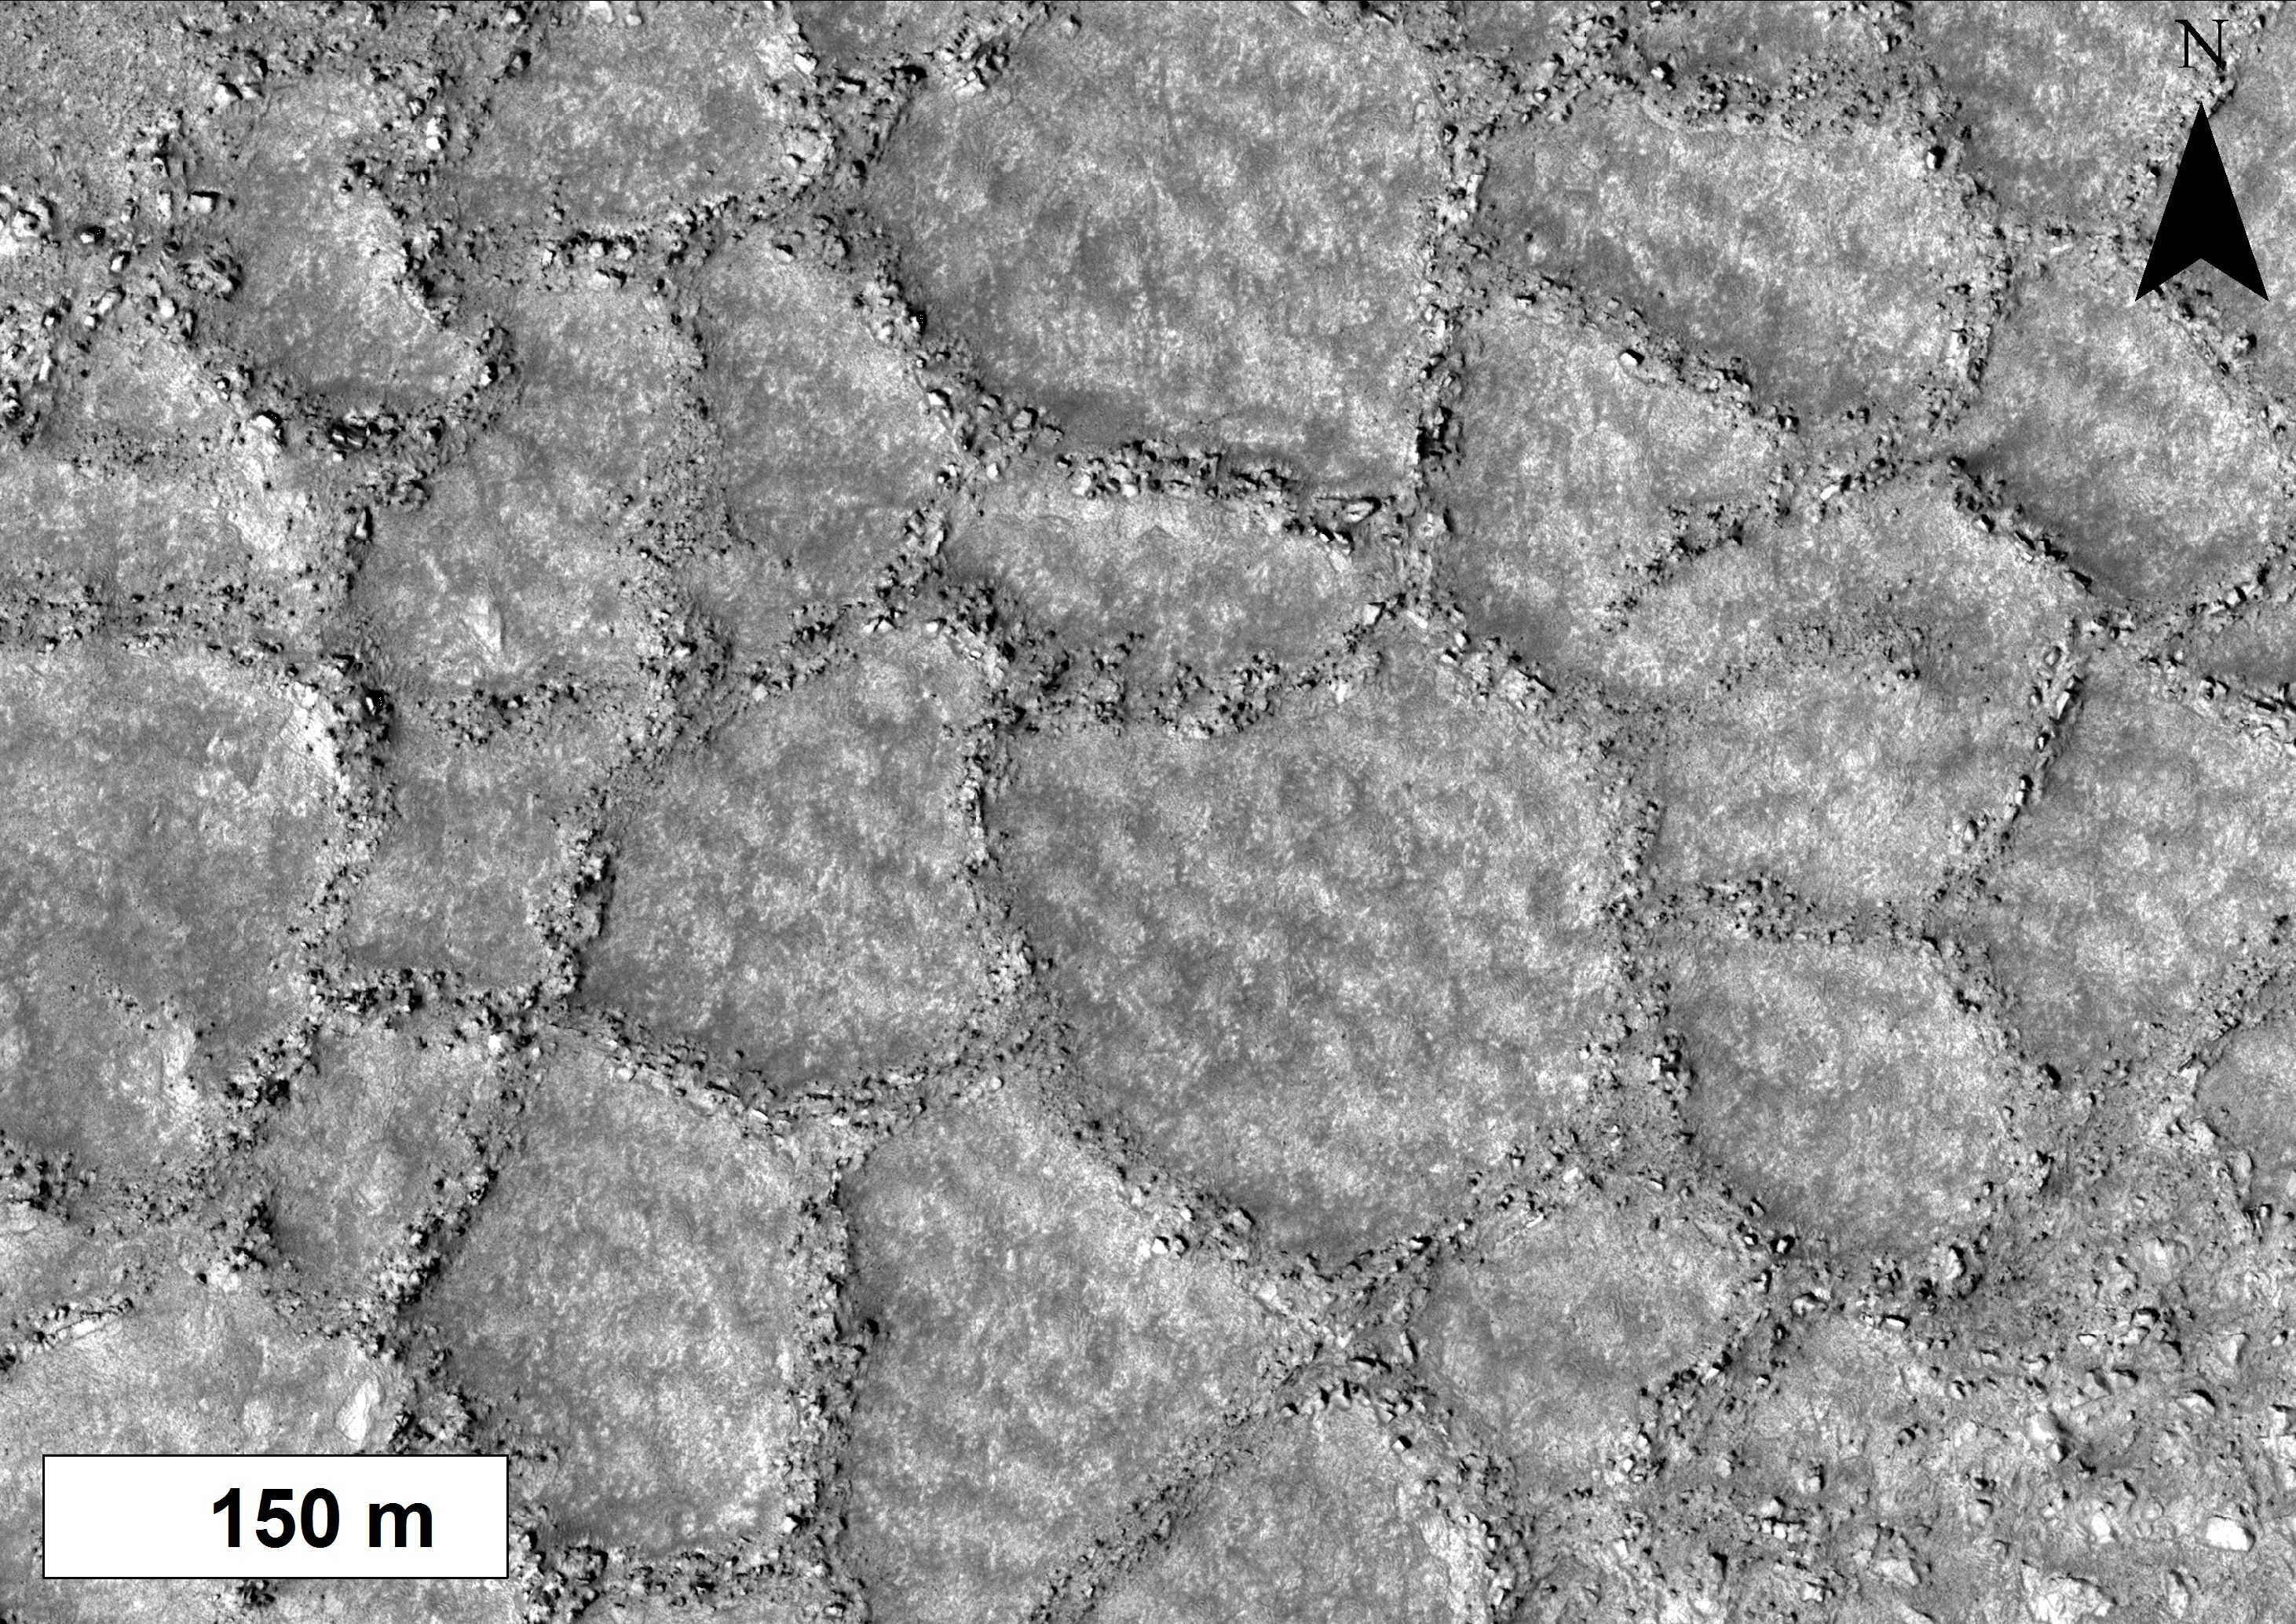
\includegraphics[width=0.5\linewidth]{images/polygonal.jpg}
    \caption{Polygonal ground observed to the north east of Lyot crater, Mars.}
    \label{fig:enter-label}
\end{figure}

Dust is a particularly persistent geologic hazard. Dust accumulation on solar panels can significantly degrade power generation efficiency over time. It can also interfere with sensor optics and thermal radiators, affecting both instrument performance and thermal control. Dust mitigation strategies, such as electrostatic dust removal or mechanical cleaning mechanisms, may be necessary depending on mission duration and power architecture\footnote{See \cite{nasa_2019_env_hazards}}.

\subsection*{Atmospheric Hazards}

While the Martian atmosphere is very thin (approximately 0.6\% of Earth’s surface pressure), it can still support dynamic weather phenomena, including dust devils, regional dust storms, and seasonal winds\footnote{See \cite{asu_2019_atmosphere}}. These phenomena introduce potential hazards to the mission in several ways:

\begin{itemize}
    \item \textbf{Dust storms:} While global storms are relatively rare, regional storms can obscure sunlight for days or weeks, disrupting solar power systems and reducing thermal regulation capability.
    \item \textbf{Wind-driven erosion:} Windborne particulates may abrade external instrument surfaces or camera lenses over time, degrading image quality or sensor calibration.
    \item \textbf{Temperature fluctuations:} Day-night temperature swings of 60--100°C are common and can induce thermal stress on instruments, cables, and joints. Thermal control systems must be robust and responsive\footnote{See \cite{nasa_2019_env_hazards}}.
\end{itemize}

\subsection*{Radiation Hazards}

Mars lacks a strong global magnetic field and has only a very thin atmosphere, offering limited protection from solar energetic particles (SEPs) and galactic cosmic rays (GCRs)\footnote{See \cite{nrc_2002_safe}}. While short-duration robotic missions may not be highly susceptible to cumulative radiation damage, sensitive electronics and any biological payloads, such as the astrobiology experiment included in this mission, must be shielded appropriately.

Radiation-induced degradation of sensors, memory storage devices, or microprocessors is a risk, especially during periods of solar activity. The rover's avionics should be radiation-hardened where possible, and scientific instruments must be qualified to withstand expected radiation doses over the planned mission duration\footnote{See \cite{nasa_2019_env_hazards}}.

\subsection*{Planetary Protection and Forward Contamination}

To prevent harmful Earth microbes from contaminating Mars or other celestial bodies, planetary protection measures must be followed. The spreading of terrestrial organisms to other planets is called forward contamination, while the reverse is known as back contamination.

Mars surface missions are designated COSPAR Category IV due to the potential for habitable environments. Accordingly, missions must follow NASA-STD-8719.27, the Planetary Protection Standard released in 2022, which outlines the bioburden control and sterilization protocols necessary to avoid compromising future life-detection science\footnote{See \cite{nasa_sma_2022_protection}}.

\subsection*{Science Goals and Risk}

There is an inherent trade-off between ensuring safety and achieving scientific objectives. Mars’ most promising sites, including ancient lake beds and volcanic terrains, are often the riskiest to explore. Addressing these hazards requires contingency planning and redundancy, such as robust systems or timeline margins.

Ultimately, the goal is to engineer for resilience, not perfection. Geologically rich but hazardous sites—like steep slopes or volatile deposits—can yield high scientific return. To explore them safely, scientists and engineers must collaborate to design adaptable systems and flexible operations, accepting that risk is an inseparable part of discovery\footnote{See \cite{nasa_2019_env_hazards}}.

\subsection*{Summary}

The Martian surface poses multiple environmental hazards that directly influence the design of the rover, instrument suite, power systems, and science operations. These include:

\begin{itemize}
    \item Rough, variable terrain that challenges mobility
    \item Dust accumulation and transport that affect power and instrumentation
    \item Atmospheric effects like dust storms, wind erosion, and temperature swings
    \item Radiation exposure that threatens electronic components and biological payloads
    \item Planetary protection requirements for astrobiology-related hardware
\end{itemize}

Mitigating these risks will require integrated engineering responses, such as mobility planning, dust-tolerant hardware, robust thermal and radiation protection, and strict adherence to contamination control protocols. Understanding and preparing for these hazards is critical to ensuring mission success and scientific return.